% select subfiles base file
\documentclass[TGAI_Laborbericht.tex]{subfiles}
\begin{document}


\chapter{Versuch 1}
\label{chap:VERSUCH_1}


\section{Fragestellung, Messprinzip, Aufbau, Messmittel}
\label{chap:VERSUCH_1_FRAGESTELLUNG}
\subsection{Fragestellung}
Im Ersten Versuch sollen wir das Windowing, welches wir in der Vorlesung kennen gelernt haben implementieren.


\subsection{Messmittel}
Als Messmittel dient ein 250g schweres Dynamisches Mikrofon mit einer Tauchspule (engl.
moving coil). Es ist Uni-direktional und reagiert auf Frequenzen im Bereich von 70Hz
bis 13 KHz und hat eine Sensitivität von -54dB ± 3dB. Die Ausgangs impendanz beträgt
500Ω±30%.

\subsection{Messprinzip}
Das Tauchspulenmikrofon (auch Tauchspulmikrofon) ist ein elektroakustischer Wandler, der
nach dem elektroinduktiven Prinzip des dynamischen Mikrofons arbeitet. Es ist sowohl die
Bauform des Druckgradientenmikrofons als auch die des Druckmikrofons üblich.
Der Begriff Tauchspulenmikrofon bezieht sich auf die technische Anordnung der Bauele-
mente des Wandlers: Bei dem Tauchspulenmikrofon ist die Membran fest mit einer Magnet-
Spule verbunden, die durch die Membranbewegung in ein statisches dauermagnetisches Feld
„eintaucht“. Siehe auch: Tauchspule. Die relative Bewegung von Spule und Magnetfeld er-
zeugt per Induktion die Signalspannung. Diese ist proportional zur Membrangeschwindig-
keit.
2
Tauchspulenmikrofone benötigen keine nachträgliche Impedanzanpassung und auch kei-
ne Symmetrierung; beides kann allein durch die Dimensionierung und Verschaltung der Spu-
le erreicht werden.
Prinzipielle Nachteile: Die Schallwelle muss die Masse der Membran mit der Spule be-
wegen und elektrische Arbeit leisten. Tauchspulenmikrofone haben daher eine geringe Emp-
findlichkeit und zeigen eine Trägheit im Einschwingverhalten, wodurch feinste Details nicht
erfasst werden, was jedoch erwünscht sein kann: Sie liefern ein „erdiges“, kräftiges Klang-
bild, hochwertige Modelle werden daher durchaus auch bei Studioaufnahmen verwendet.
Tauchspulenmikrofone haben ein nicht so hohes Übertragungsspektrum wie Kondensator-
mikrofone und sind aufgrund ihrer geringen Empfindlichkeit für Fernaufnahmen ungeeig-
net. Die relativ hohe Masse des Membransystems lässt sie zudem empfindlich auf Körper-
schall, etwa Hantierungsgeräusche, reagieren; um solche Störungen zu verringern, ist bei
hochwertigen Tauchspulenmikrofonen die gesamte technische Einheit (die Mikrofonkapsel)
im Mikrofongehäuse schwingfähig gelagert.
Die Vorteile dieses Mikrofontyps zeigen sich darin, dass sie in der Regel gegenüber me-
chanischen Belastungen recht robust sind und hohe Schalldrücke vertragen. Auch benötigen
sie keine Spannungsversorgung, was im mobilen Betrieb von Vorteil sein kann. Die einfache
Bauart erlaubt preisgünstige Fertigung und macht diesen Mikrofontyp nahezu unverwüstlich.

\subsection{Aufbau}
Das Mikrofon ist mithilfe eines Audiokabels mit der Soundkarte des Laborrechners verbunden.



\section{Messwerte}
\label{chap:VERSUCH_1_MESSWERTE}
Zuerst schreiben wir uns ein python skript, in welchenm wir mithilfe des Moduls Pyaudio ein Signal aufnehmen. Zur Hilfe haben wir hier das Skript von J. Keppler aus der Moodle einführung. Dieses Signal speichern wir dann mit der Funktion numpy.save() ab. Nun erweitern wir das Programm noch um eine Triggerfunktion. Wir haben uns dafür entschieden, dass das Signal erst ab einem bestimmten Amplitudenwert aufnimmt. So ist sichergestellt, dass erst sobald man in das Mikrofon reinspricht, das Programm auch mit der Aufnahme beginnt. Nun stellen wir die Aufnahmelänge noch auf eine Sekunde ein.

\section{Auswertung}
\label{chap:VERSUCH_1_AUSWERTUNG}
Nachdem wir das Signal aufgenommen haben, errechnen wir nun noch mithilfe der Funktion numpy.fft.fft() das Amplitudenspektrum. Nun wenden wir noch das Windowing, welches wir in der Vorlesung kennengelernt haben an. Hierzu zerlegen wir das Signal in kleine Fenster von einer Länge von 512 samples. Diese Fenster müssen sich auch überlappen, hierzu nehmen wir die Hälfte des Vorherigen bzw nächsten Fensters. Auf das jeweilige Fenster multiplizieren wir jetzt noch die Gaußchen Fensterfunktion bei welcher die Fensterbreite der 4fachen Standardabweichung entspricht Hieraus berechnen wir nun wieder das Spektrum.

\begin{figure}[H]
	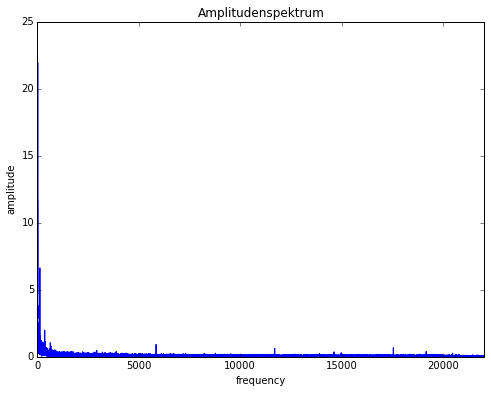
\includegraphics[width=0.7\textwidth]{media/amplitudenspektrum.png}
	\label{Amplitudenspektrum}
	\caption{Amplitudenspektrum}
\end{figure}

\begin{figure}[H]
	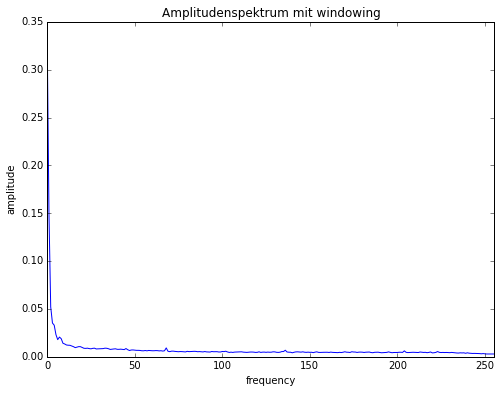
\includegraphics[width=0.7\textwidth]{media/windowing.png}
	\label{Windowing}
	\caption{Windowing}
\end{figure}




\section{Interpretation}
\label{chap:VERSUCH_1_INTERPRETATION}
Nun haben wir eine Aufnahmefunktion, um die Referenzen für Aufgabe 2 aufzunehmen. Nebenbei haben wir noch das Windowing angewandt, mithilfe des Windowing bekommen wir eine genauere Auflösung des Frequenzbandes. Siehe Komplementarität von Frequenz und Zeit. 
\end{document}

